\chapter{Results}\label{ch:results}

During the training and testing stages, a number of plots have been made in order to visualize any outliers, along with a list of any anomalies the network has found. Note that these plots and anomalies are all based on 1\% of the users.

\begin{figure}
	\begin{center}
		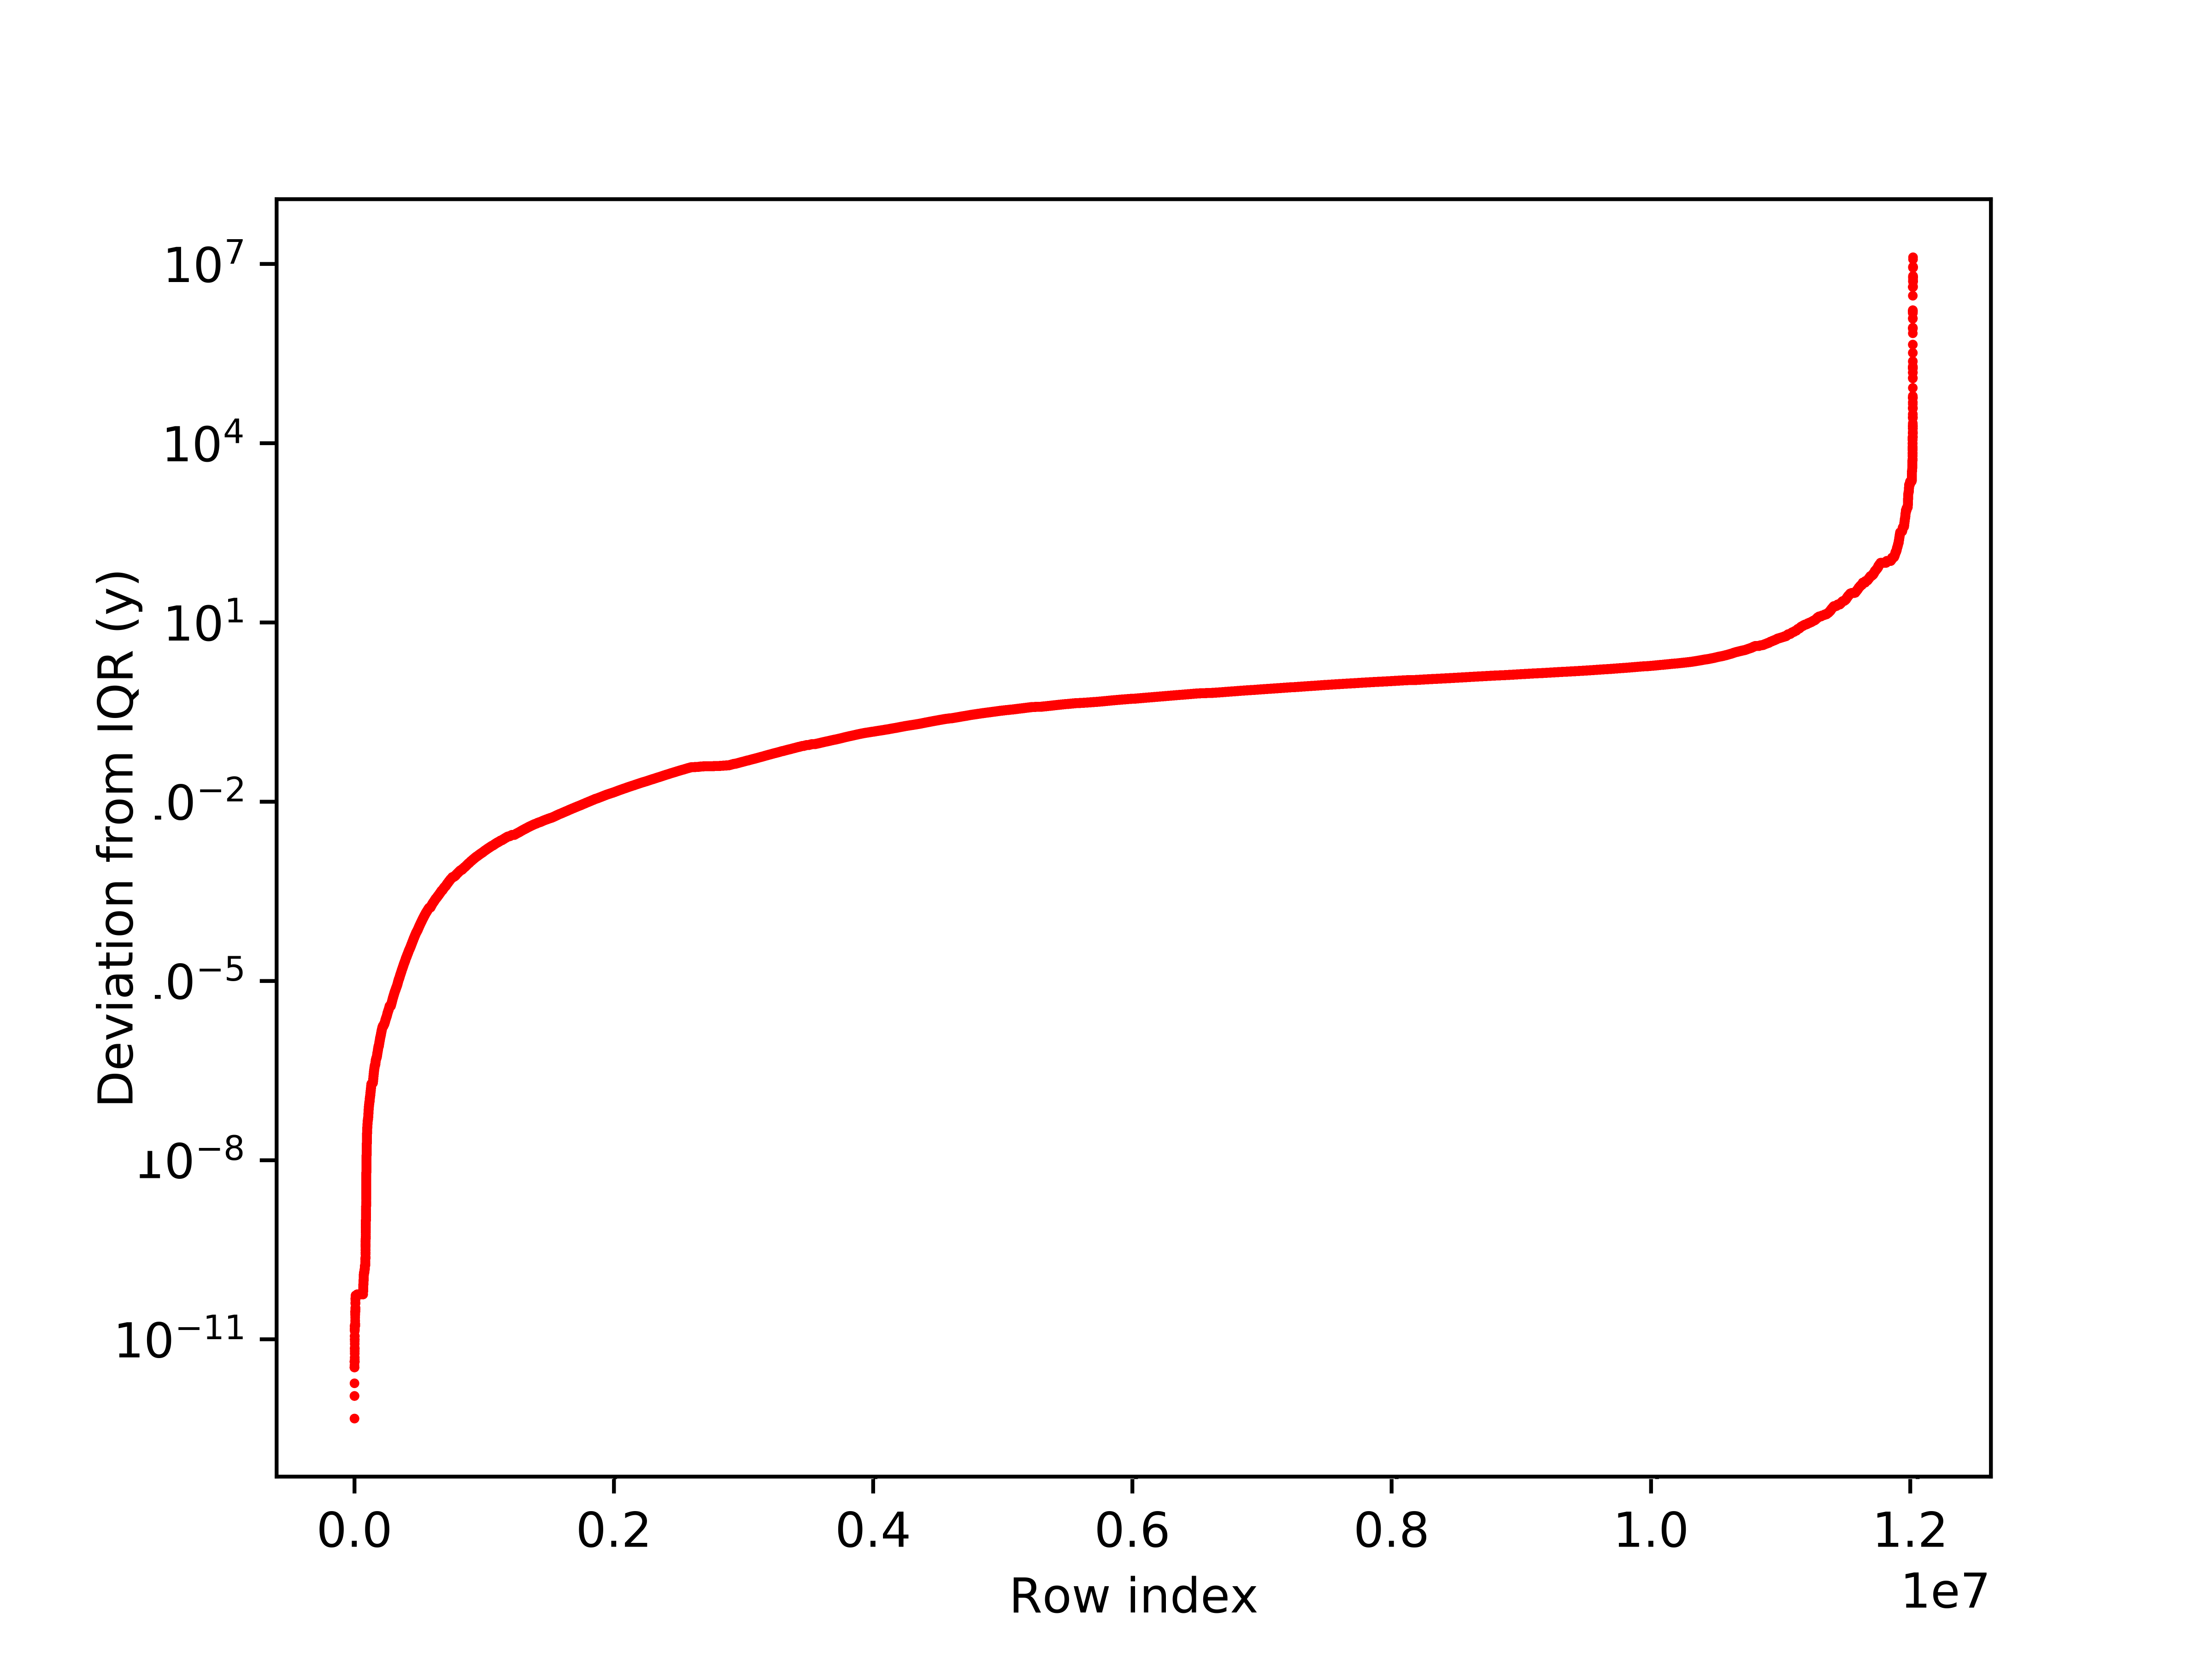
\includegraphics[scale=0.1]{results/all_deviations}
	\end{center}
	\caption{The deviations \(y\) (function ~\ref{eq:y}) of the mean squared errors of all predicted test set feature vectors compared to the actual feature vectors. The IQR has been calculated over the training set using the same method of predicted vs actual mean squared error.~\label{fig:iqr_scale}}
\end{figure}

In order to get an idea of how much the error between the predicted feature vector and the actual feature vector deviates from that user's mean error, a function has been created with which this can be calculated. When replacing 1.5 with \(y\) in equation~\ref{eq:iqr_max}, with \(x\) being the mean squared error (function~\ref{eq:mse}) between the predicted feature vector and the actual feature vector, solving for \(y\) gives the following function:

\begin{equation} \label{eq:y}
y = (x - Q3) / IQR
\end{equation}

This \(y\) value is then plotted, the result of which can be seen in figure~\ref{fig:iqr_scale}. As can be seen in the figure, there are quite a number of outliers, some of which having IQR-scores that fall far beyond the cutoff value of 1.5. From this, it can be concluded that at least some outliers are being found. 

\begin{figure}
	\begin{center}
		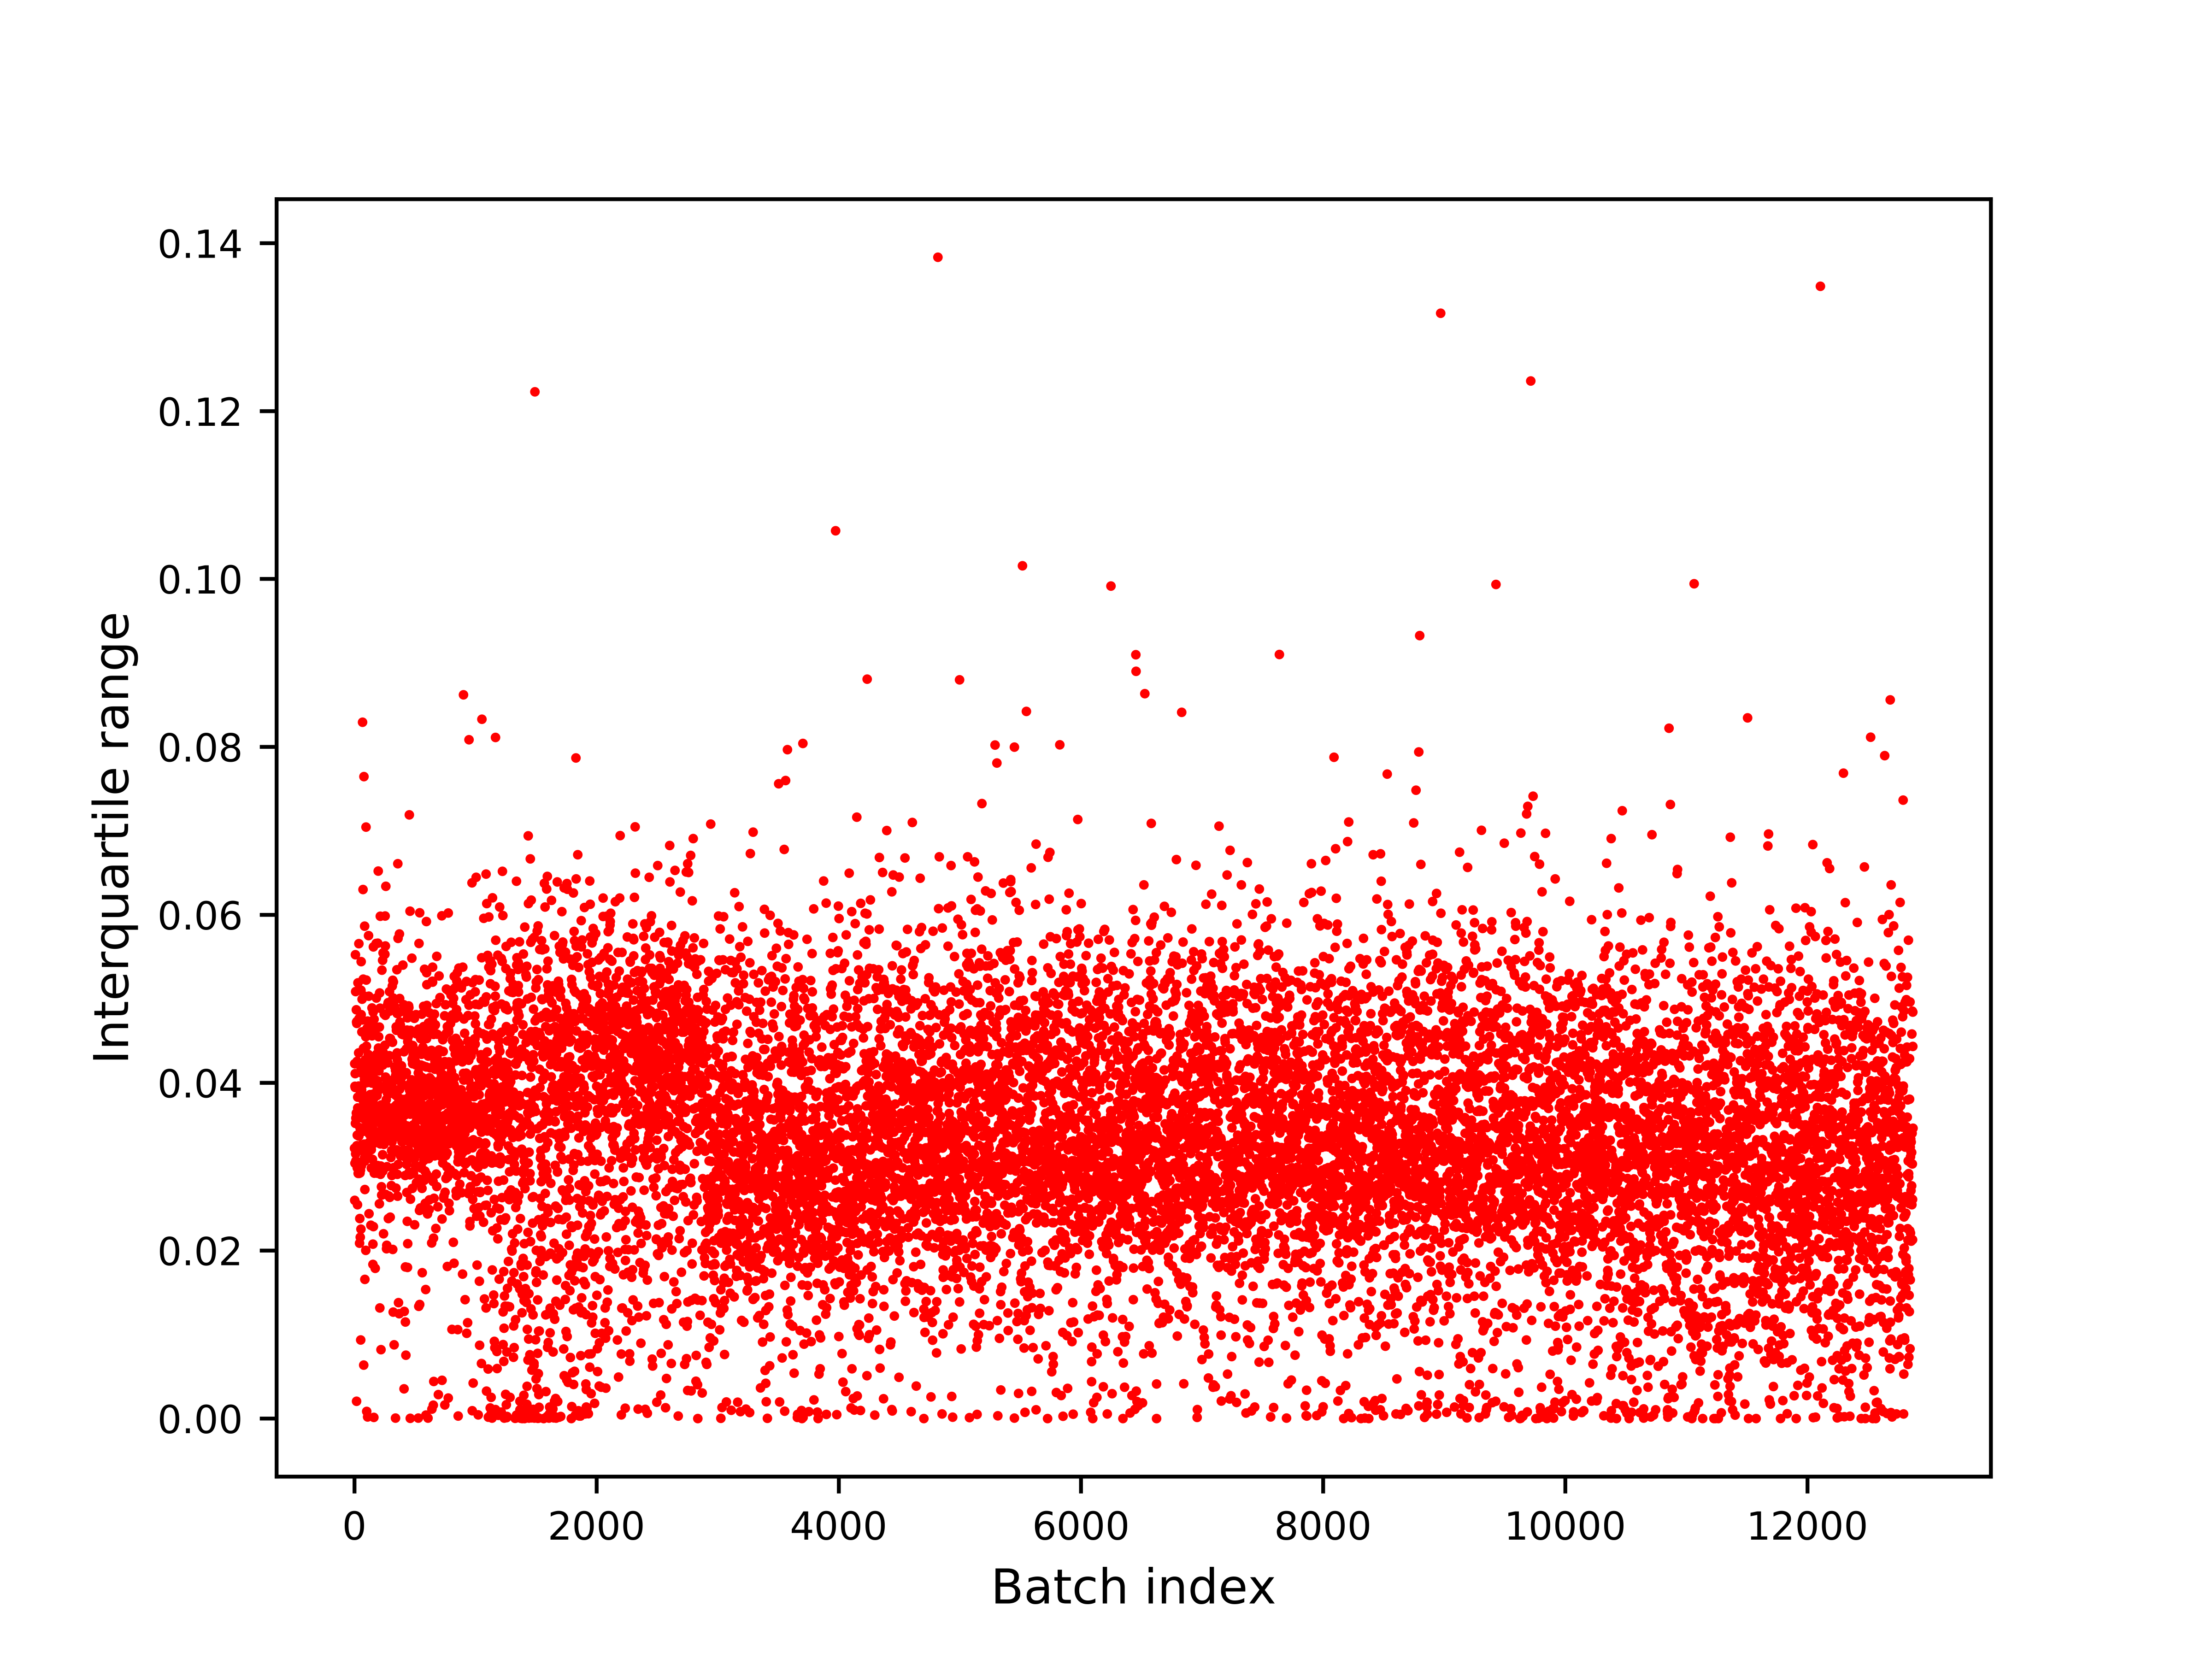
\includegraphics[scale=1.6]{results/iqrs}
	\end{center}
	\caption{The IQR values calculated over the mean squared errors of all test set feature vectors and their predictions, by user. Note that for actual testing, the IQR is calculated over the training set, this is simply done to show the distribution of the losses of all users.~\label{fig:iqrs}}
\end{figure}

As can be seen in figure~\ref{fig:iqrs}, the IQRs tend to be fairly close to each other, meaning the mean losses are close to each other as well. This shows that the network is relatively successful at modeling user behavior, as the difference between the expected and actual action calculated by the loss function shows few big spikes. A network that is unsuccessful at this would have inconsistent IQRs as the losses would fluctuate more from user to user and would show higher values indicating bad predictions.

\begin{figure}
	\begin{center}
		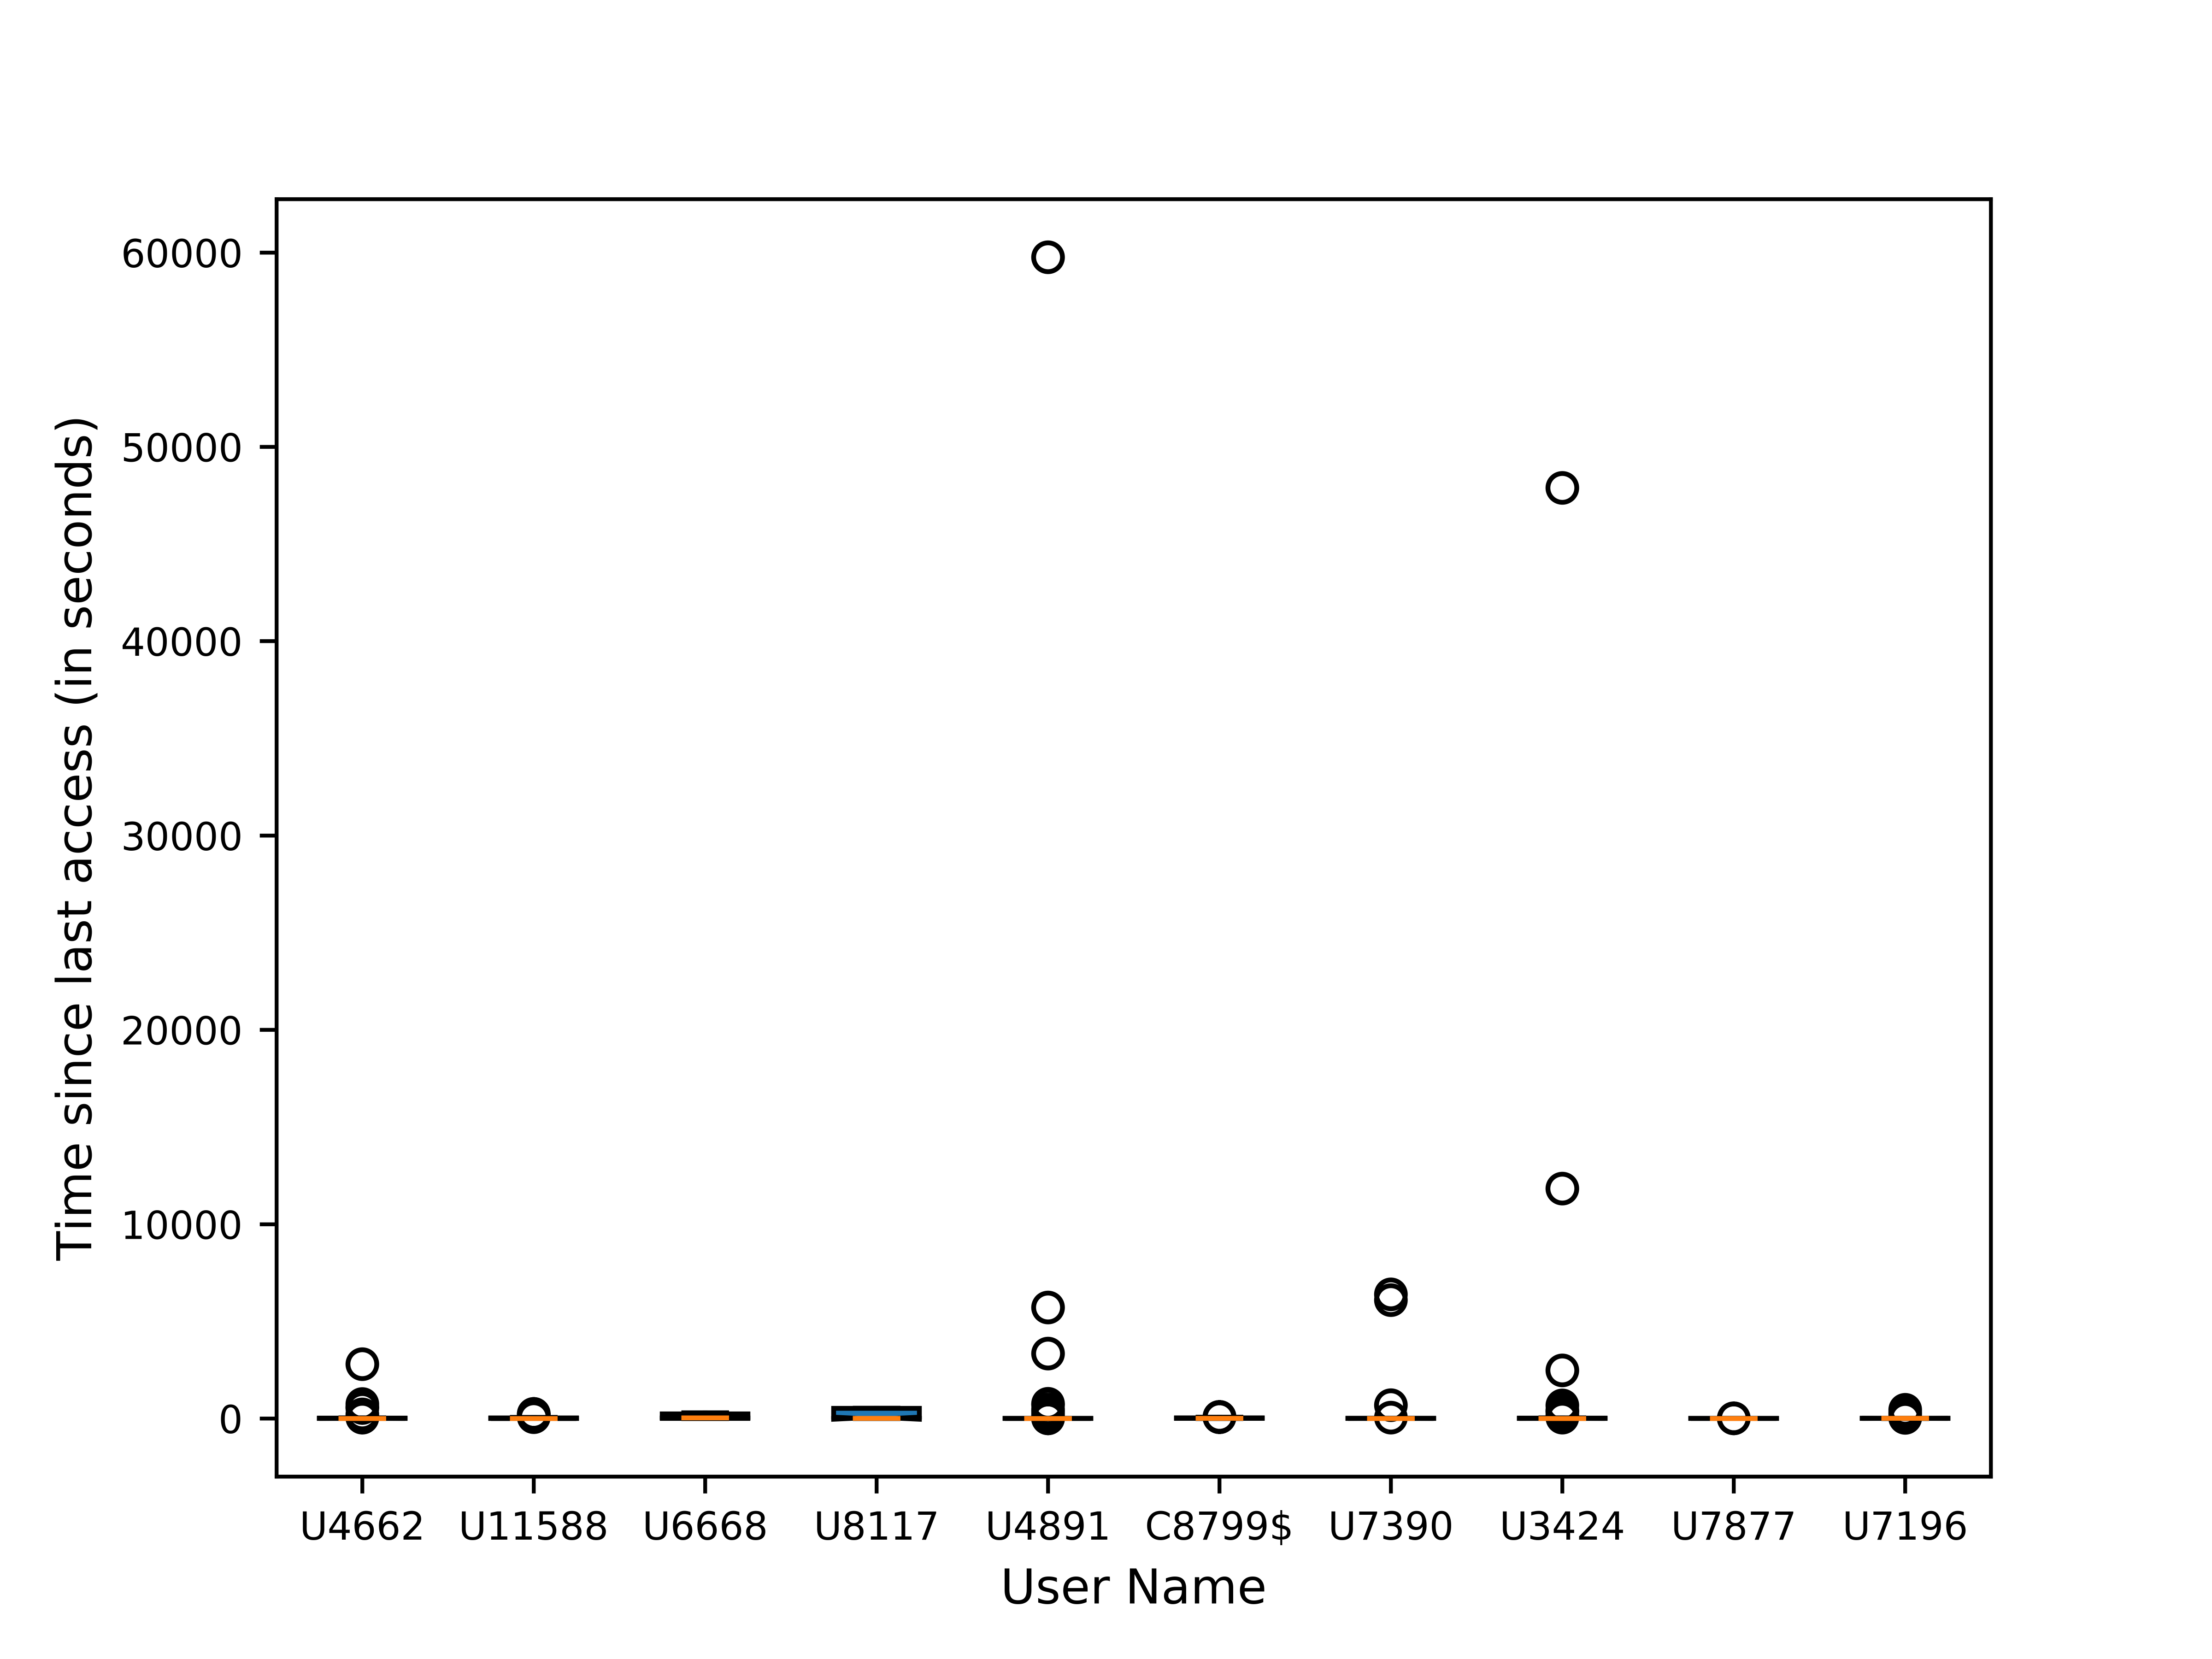
\includegraphics[scale=1.6]{results/highest_offender_time_since_last_access}
	\end{center}
	\caption{The top 10 highest offenders' seconds since last access.~\label{fig:time_since_last_access}}
\end{figure}

Focussing on the highest offending users allows us to see more clearly why the network thought certain users were deemed anomalies and whether the network may have been right.

In figure~\ref{fig:time_since_last_access} a closer look is taken at the time since the last network access for the top 10 highest offending users. This clearly shows some very big deviations from users' times since their last network access. For example, U41 consistently has a very low time since last access, as can be seen from the box plot being very small and concentrated around that area. However, there is a significant deviation from this user's normal behavior, which the network has probably flagged as a deviation. The same goes for other users like U102 and U72, changing their behavior a lot, while \enquote{normal} users like U34, U107 and U119 keep their time since last access consistent. U41's pause only took 2 weeks, which can easily be explained by a vacation, a period of sickness or any other reason for taking a short break. However, this is something that is still worth investigating, as this could also be an abandoned account being picked up by a different (potentially malicious) user.

\begin{table}[htbp]
	\centering
	\caption{The predicted features vs the actual features of the top offending feature set by U399 (precise to 3 decimals)}\label{tab:predicted_vs_actual_top}
	\begin{tabular}{lll}
		Label & Actual & Predicted \\ \midrule
		time\_since\_last\_access & 0.060 & 0.011 \\
		domains\_delta & 0 & 0.000 \\
		dest\_users\_delta & 1 & 0.000 \\
		src\_computers\_delta & 1 & 0.000 \\
		dest\_computers\_delta & 1 & 0.000 \\
		percentage\_failed\_logins & 0.001 & 0.000 \\
		success\_failure & 1 & 0.999 \\
		auth\_type\_0 & 0 & 0.000 \\
		auth\_type\_1 & 0 & 1.000 \\
		auth\_type\_2 & 0 & 0.000 \\
		auth\_type\_3 & 0 & 0.000 \\
		auth\_type\_4 & 0 & 0.000 \\
		auth\_type\_5 & 0 & 0.000 \\
		auth\_type\_6 & 0 & 0.000 \\
		auth\_type\_7 & 0 & 0.000 \\
		auth\_type\_8 & 0 & 0.000 \\
		auth\_type\_9 & 1 & 0.000 \\
		auth\_type\_10 & 0 & 0.000 \\
		logon\_type\_0 & 0 & 0.000 \\
		logon\_type\_1 & 0 & 0.000 \\
		logon\_type\_2 & 0 & 0.000 \\
		logon\_type\_3 & 0 & 0.999 \\
		logon\_type\_4 & 0 & 0.000 \\
		logon\_type\_5 & 0 & 0.000 \\
		logon\_type\_6 & 0 & 0.000 \\
		logon\_type\_7 & 1 & 0.000 \\
		logon\_type\_8 & 0 & 0.000 \\
		auth\_orientation\_0 & 0 & 0.999 \\
		auth\_orientation\_1 & 0 & 0.000 \\
		auth\_orientation\_2 & 1 & 0.000 \\
		auth\_orientation\_3 & 0 & 0.000 \\
		auth\_orientation\_4 & 0 & 0.000 \\
		auth\_orientation\_5 & 0 & 0.000
	\end{tabular}
\end{table}

\begin{table}[htbp]
	\centering
	\caption{The highest offending user's last 30 logins before the anomaly and the anomaly last}\label{tab:prev_logins}
	\resizebox{\linewidth}{!}{
		\begin{tabular}{lllllllll}
			time (ms) & source user@domain & destination user@domain & source computer & destination computer & authentication type & logon type & authentication orientation & success/failure \\ \midrule
			3769690 & U399@DOM5 & U400@C832 & C832 & C832 & Negotiate & Interactive & LogOn & Success \\
			3769706 & U399@DOM5 & U400@C832 & C832 & C832 & Negotiate & Interactive & LogOn & Success \\
			3769720 & U399@DOM5 & U400@C832 & C832 & C832 & Negotiate & Interactive & LogOn & Success \\
			3769728 & U399@DOM5 & U400@C832 & C832 & C832 & Negotiate & Interactive & LogOn & Success \\
			3769732 & U399@DOM5 & U400@C832 & C832 & C832 & Negotiate & Interactive & LogOn & Success \\
			3769734 & U399@DOM5 & U400@C832 & C832 & C832 & Negotiate & Interactive & LogOn & Success \\
			3769750 & U399@DOM5 & U400@C832 & C832 & C832 & Negotiate & Interactive & LogOn & Success \\
			3769753 & U399@DOM5 & U400@C832 & C832 & C832 & Negotiate & Interactive & LogOn & Success \\
			3769754 & U399@DOM5 & U400@C832 & C832 & C832 & Negotiate & Interactive & LogOn & Success \\
			3769755 & U399@DOM5 & U400@C832 & C832 & C832 & Negotiate & Interactive & LogOn & Success \\
			3769769 & U399@DOM5 & U400@C832 & C832 & C832 & Negotiate & Interactive & LogOn & Success \\
			3769811 & U399@DOM5 & U400@C832 & C832 & C832 & Negotiate & Interactive & LogOn & Success \\
			3769849 & U399@DOM5 & U400@C832 & C832 & C832 & Negotiate & Interactive & LogOn & Success \\
			3769861 & U399@DOM5 & U400@C832 & C832 & C832 & Negotiate & Interactive & LogOn & Success \\
			3770055 & U399@DOM5 & U400@C832 & C832 & C832 & Negotiate & Interactive & LogOn & Success \\
			3770057 & U399@DOM5 & U400@C832 & C832 & C832 & Negotiate & Interactive & LogOn & Success \\
			3770058 & U399@DOM5 & U400@C832 & C832 & C832 & Negotiate & Interactive & LogOn & Success \\
			3770066 & U399@DOM5 & U400@C832 & C832 & C832 & Negotiate & Interactive & LogOn & Success \\
			3770112 & U399@DOM5 & U400@C832 & C832 & C832 & Negotiate & Interactive & LogOn & Success \\
			3770113 & U399@DOM5 & U400@C832 & C832 & C832 & Negotiate & Interactive & LogOn & Success \\
			3770114 & U399@DOM5 & U400@C832 & C832 & C832 & Negotiate & Interactive & LogOn & Success \\
			3770115 & U399@DOM5 & U400@C832 & C832 & C832 & Negotiate & Interactive & LogOn & Success \\
			3770116 & U399@DOM5 & U400@C832 & C832 & C832 & Negotiate & Interactive & LogOn & Success \\
			3770144 & U399@DOM5 & U400@C832 & C832 & C832 & Negotiate & Interactive & LogOn & Success \\
			3770146 & U399@DOM5 & U400@C832 & C832 & C832 & Negotiate & Interactive & LogOn & Success \\
			3770148 & U399@DOM5 & U400@C832 & C832 & C832 & Negotiate & Interactive & LogOn & Success \\
			3770152 & U399@DOM5 & U400@C832 & C832 & C832 & Negotiate & Interactive & LogOn & Success \\
			3770154 & U399@DOM5 & U400@C832 & C832 & C832 & Negotiate & Interactive & LogOn & Success \\
			3770156 & U399@DOM5 & U400@C832 & C832 & C832 & Negotiate & Interactive & LogOn & Success \\
			3770158 & U399@DOM5 & U400@C832 & C832 & C832 & Negotiate & Interactive & LogOn & Success \\
			3770158 & U399@DOM5 & U400@C832 & C832 & C832 & MICROSOFT_AUTHENTICATION_PA & REMOTEINTERACTIVE & TGS & Success
		\end{tabular}
	}
\end{table}

The highest offending (highest mean squared error value) feature vector's predicted vs actual action are shown in Table~\ref{tab:predicted_vs_actual_top}. In this table (and following tables) features that are integers and not floats have been depicted as integers, as all but the \(percentage\_failed\_logins\) and \(time\_since\_last\_access\) features are integers. Any predictions made by the network are trimmed to 3 decimal points.

%cSpell:words REMOTEINTERACTIVE
As can be seen, the action itself isn't very weird, simply using a different method of authentication, a different method of logging in and a different authentication orientation. These methods themselves are not inherently anomalies, but the network learned that these actions are rarely made by the user, assigning a value of 0.000 to \(auth\_type\_0\) (NTLM), \(logon\_type\_7\) (REMOTEINTERACTIVE) and \(auth\_orientation\_2\) (TGS). The network also assigned values of 0.999 or higher to a single action in all of these enums, pointing to the user almost always logging in using these exact methods. When compared to the user's previous logins in Table~\ref{tab:prev_logins}, the last action really stands out as different. Many anomalies like this have been found. A user often logs in after a really long time relative to their other login times or significantly changes their behavior by logging in using methods rarely or never used before. This indicates that the network is doing a good job at recognizing the user's behavior and finding anything that deviates from it.